\section{Cerberus: BB Aware Batch Scheduler}
\label{Sec:Scheduler}

\begin{figure}[!htbp]
        \centering
        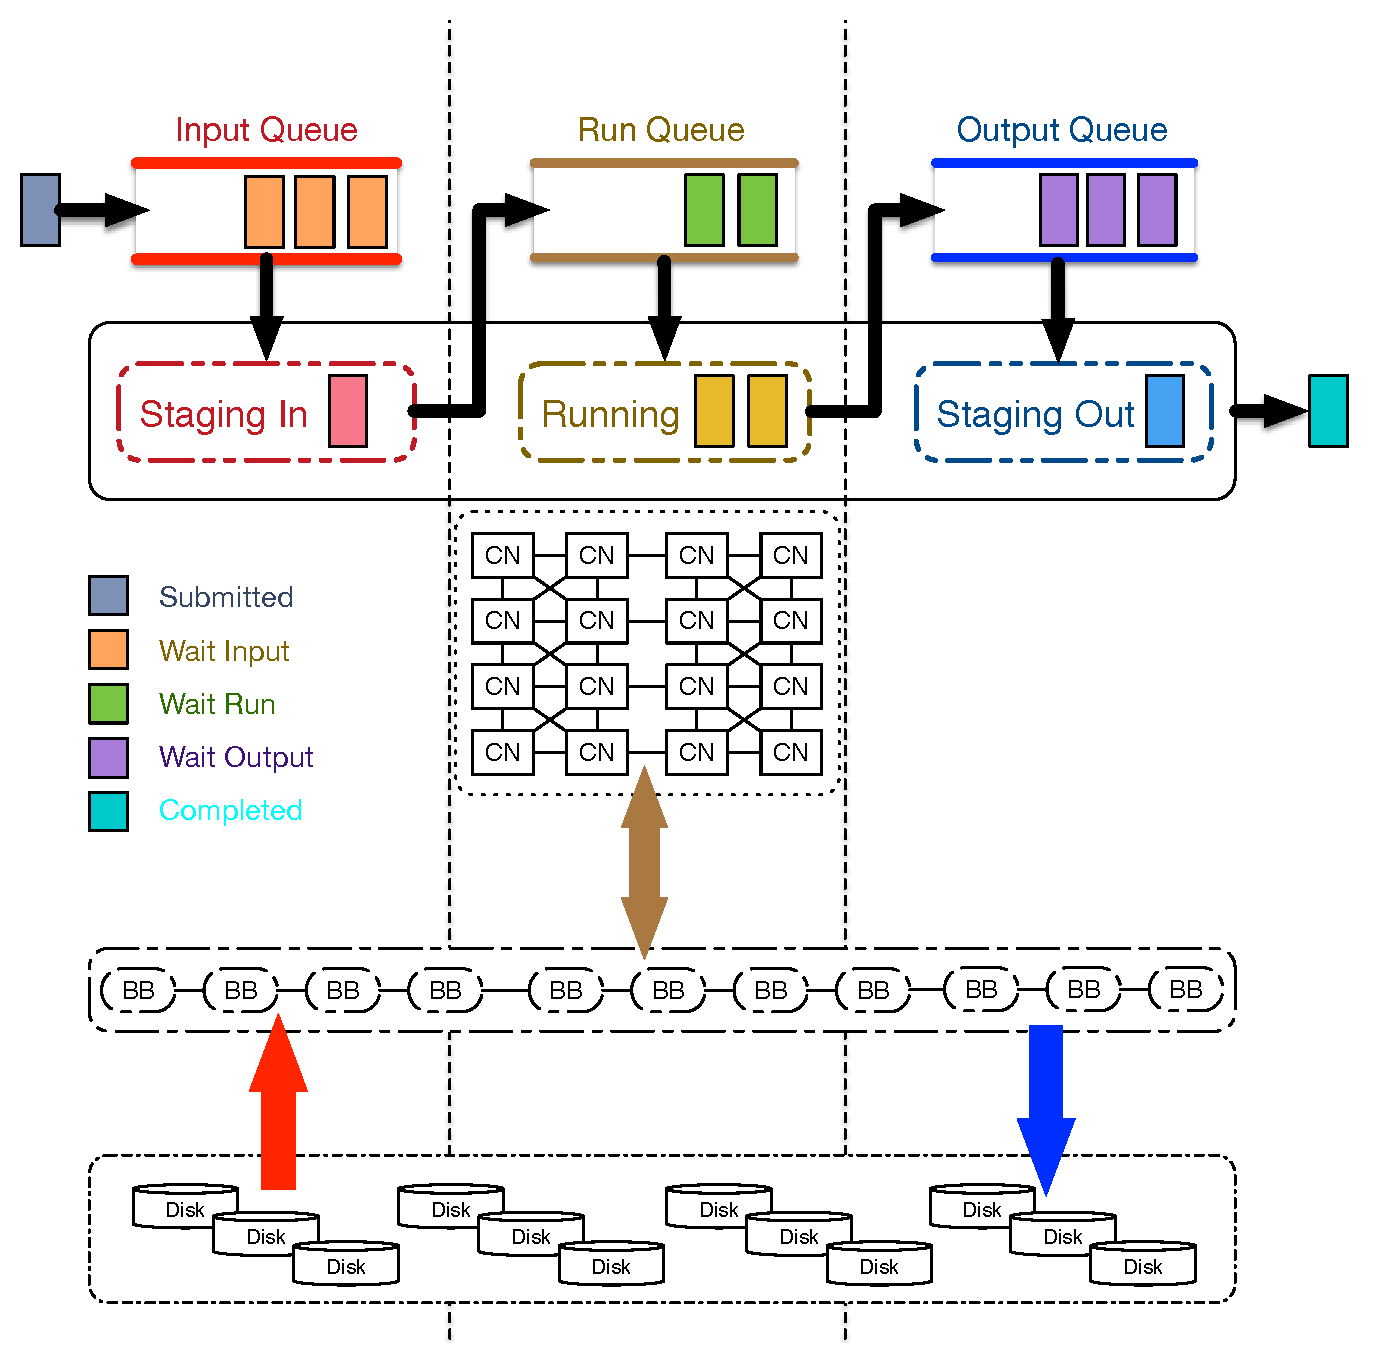
\includegraphics[width=3.6in]{CerberusBBSystem}
        \caption{Scheduling Workflow of Burst Buffer Aware Cerberus}
        \label{Fig:CerberusQueues}
\end{figure}

%=======XY======
\subsection{Cerberus Overview}

The traditional batch scheduler on system without burst buffer only
takes job size (required number of nodes) and expected runtime into scheduling decision making. 
The most commonly used scheduling policy are First Come First Serve with EASY backfilling~\cite{tsafrir-tpds-2007}.
However, on burst buffer enabled systems, 
the available amount of burst buffer capacity becomes the new scheduling constraint. 
Thus, we propose Cerberus, 
the batch scheduler with burst buffer awareness for 3-phase modeled jobs. 

% \subsection{Cerberus for 3-Phase Jobs}
% Traditional batch scheduler usually looks at the field of $c_i$ and $rt_i$
% when making scheduling decision.
% One straightforward way to make decisions on non-burst-buffer HPC system is
% First Come First Serve, as long as available compute nodes can satisfy user job.
% Once the system is equipped with burst buffer, scheduler must consider a new constraint:
% the available amount of burst buffer capacity.
% Scheduling is divided into 3 phases to
% adopt to the 3-phase characteristic of jobs in burst buffer context.
% As shown in Figure~\ref{Fig:CerberusQueues},
% Cerberus schedules jobs in 3 distinct set/queue.
% The input queue $Q_I$ contains all the jobs that
% needs to load input data before they are able to execute.
% Once a job comes out of input queue, its data flows from external disk
% to burst buffer nodes, indicated by the red arrow.
% Compute nodes are not allocated to the application until
% data flows from burst buffer to memory on compute nodes.
% The run queue $Q_R$ contains all the jobs waiting to be run with loaded data.
% Before executing, input data must be transfered to memory on compute nodes,
% after which burst buffer used for stage-in can be released.
% When running application request checkpointing, its execution and data are
% pushed to its exclusive burst buffer nodes;
% when application resume from system fault, its checkpointing are
% loaded directly from burst buffer, instead of PFS, to compute nodes.
% The output queue $Q_O$ contains all the jobs that
% terminate execution but needs to write output data to external storage.
% As soon as output data is moved from memory to burst buffer nodes allocated for stage-out,
% compute nodes can be released;
% in other words, other applications ready to run can take up them now.
% At anytime, a job can only appear in one of the 3 sets, apparently.
% This fact motivates separated scheduling idiom to be used in different phases,
% or for different job queues.

%==================XY==============================

As shown in Figure~\ref{Fig:CerberusQueues},
the input queue $Q_I$ contains all the jobs that
needs to pre-fetch data from external storage to burst buffer.
When the data flows from external disk
to burst buffer nodes, indicated by the red arrow, the job enters the run queue $Q_R$, 
waiting for compute nodes to be allocated.
Once the job gets the required number of compute nodes, it can start to run.
There might be frequent data exchange between burst buffer and compute nodes during the running phase. 
The job enters the output queue $Q_O$ after finishing computation, 
and waits for its output data being drained out to external storage. 

There could be multiple jobs waiting in each queue at the same time. 
Cerberus schedules the jobs in each queue separately, 
rather than being held in a particular queue and waiting for certain resources.

\subsection{Coordination Among Three Phases}
There are few things to notice.
First, for a given job, its three phases are temporally dependent.
That is, only after finishing stage-in phase can a job be ready for running;
similarly, only when finishing running phase can a job waiting or entering stage-out phase.
This is reflected in the lifetime of a job's execution.

Secondly, for any job,
its requested burst buffer can only be used for 1 purpose.
For example, a running-phase job cannot hold its already taken burst buffer
and use them to enter stage-out phase upon finishing running,
no matter whether $bb\_run > bb\_out$ or $bb\_run < bb\_out$.
In Cerberus, resource release must be done mandatorily as specified in section~\ref{Sec:Model},
We believe frequent release provides more opportunities to make scheduler involved in each phase of the jobs.

At last, it is possible that all 3 queues are not empty at the moment of scheduling.
We choose a heuristic strategy to determine the scheduling order when
Cerberus has to handle multiple queues at the same time.
Noticing that jobs finishing \textit{running} and \textit{stage-out} phase
will fully or partially release taken resources,
we set the priority of queues to be $priority(Q_O) > priority(Q_R) > priority(Q_I)$.
This greedy heuristic works well when the demand of jobs in $J_{Q_I}$ is low.
However, it is possible to make jobs stacking up at the entry of the system.
We plan to investigate more on this problem in the future.

\begin{figure}[!htbp]
\centering
        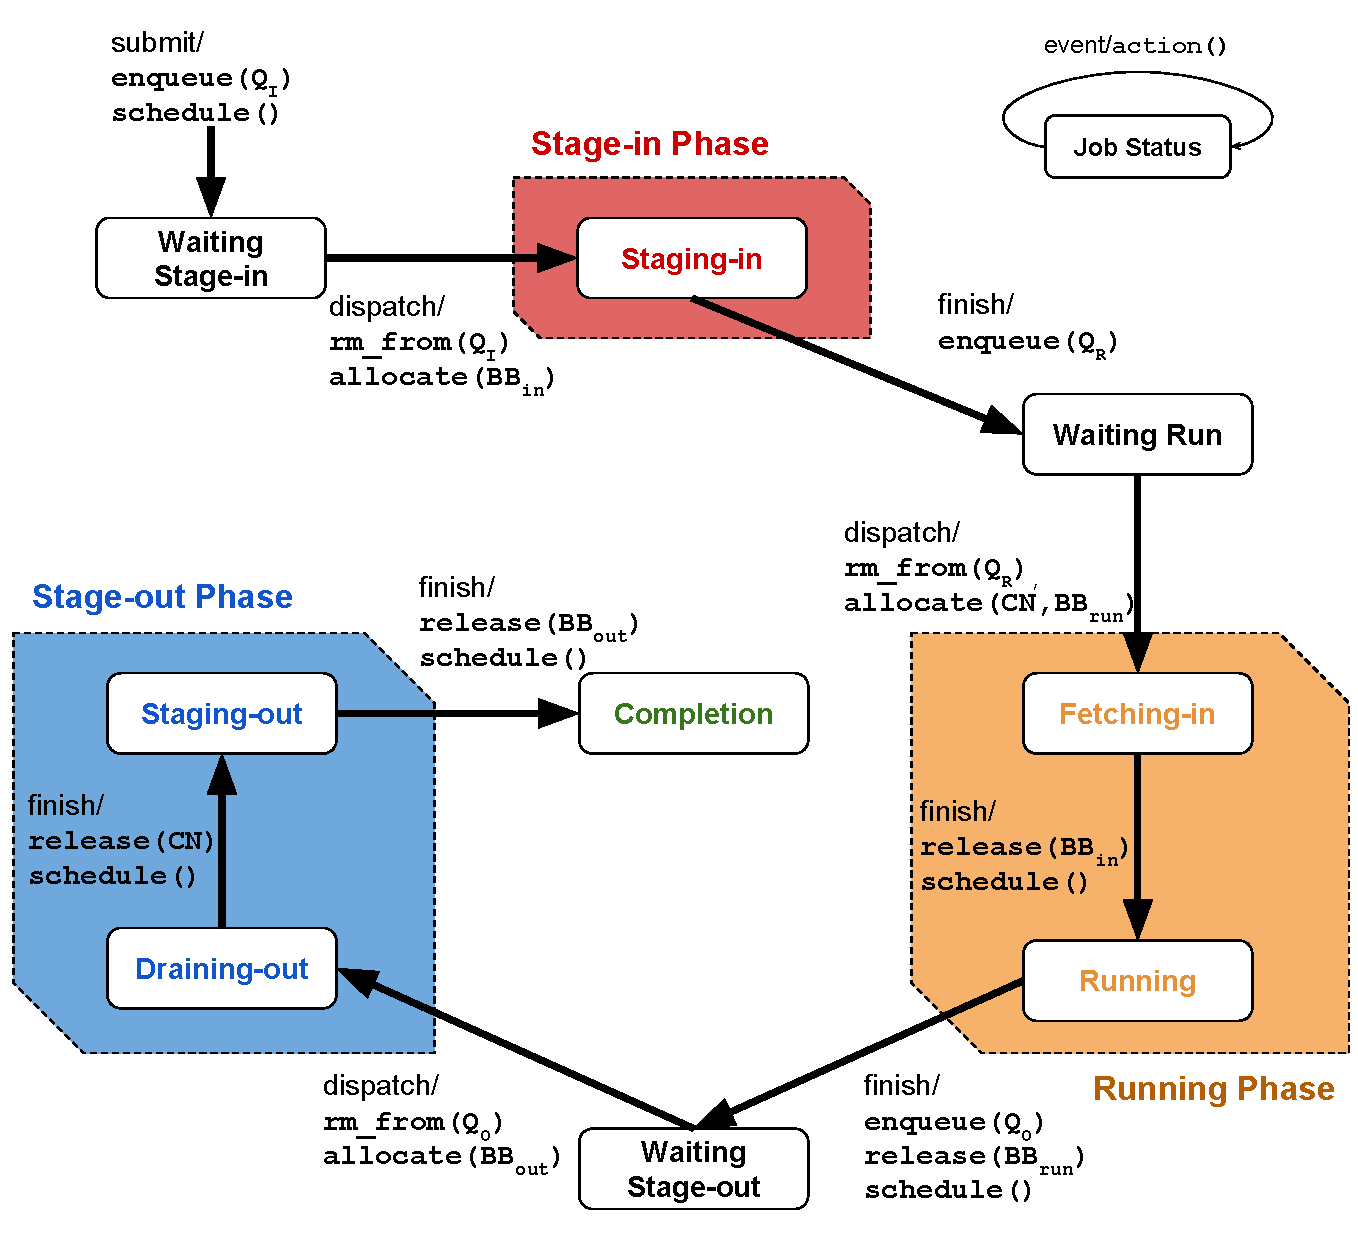
\includegraphics[width=3.6in]{3PhaseJobFSM}
        \caption{Event-driven BBsim scheduling model}
\label{Fig:JobFSM}
\end{figure}

